\documentclass[border=6mm]{standalone}

\usepackage{tikz} \usepackage[sfdefault,scaled=.85]{FiraSans}
\usepackage{newtxsf}

\usepackage[T1]{fontenc}
\begin{document}

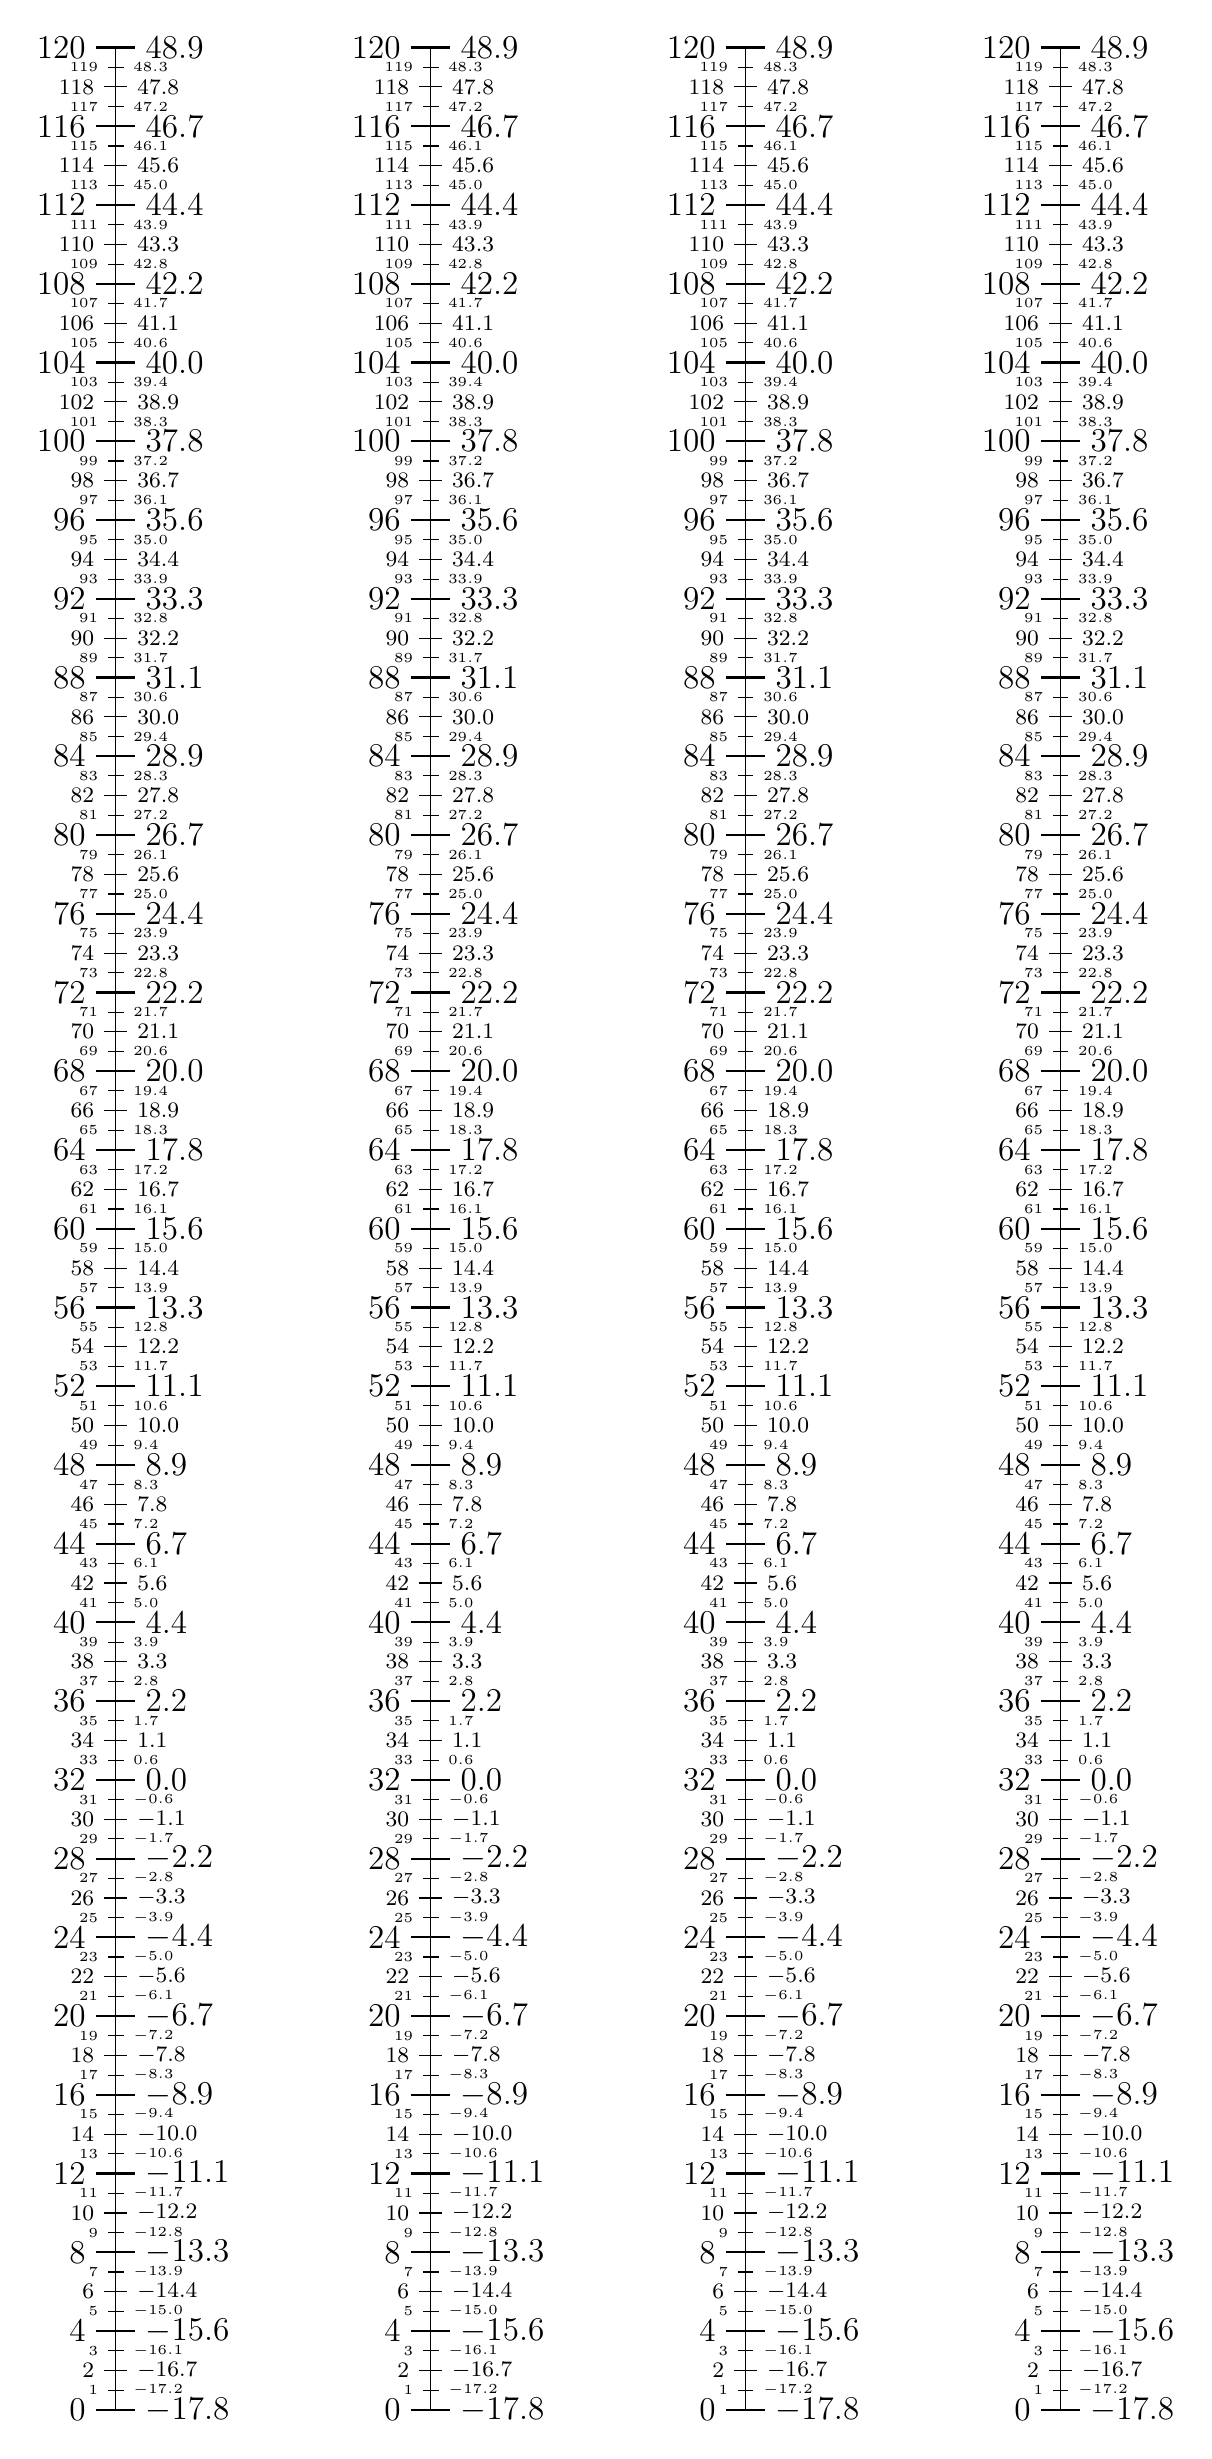
\begin{tikzpicture}[yscale=0.25]
  \foreach \j in {0,4,...,12}
  {
 \pgfkeys{/pgf/number format/.cd,std,fixed,int detect,precision=0}
\draw (\j,0)-- (\j,120);
\foreach \i in {0,4,...,120} % numbers on line
\draw[thick] (\j,\i) -- + (-0.25,0) node[left]   {\large{\pgfmathprintnumber{\i}}};
   \foreach \i in {2,6,...,118}
   \draw (\j,\i) -- + (-0.15,0) node[left] {\footnotesize{\pgfmathprintnumber{\i}}};
   \foreach \i in {1,3,...,119}
   \draw (\j,\i) -- + (-0.1,0) node[left] {\tiny{\pgfmathprintnumber{\i}}};
  
\pgfkeys{/pgf/number format/.cd,std,fixed,zerofill=true,precision=1}
\foreach \i in {0,4,...,120} % numbers on line
\draw[thick] (\j,\i) -- + (0.25,0) node[right] {\large{\pgfmathparse{(\i-32)*5/9}\pgfmathprintnumber{\pgfmathresult}}};

\foreach \i in {2,6,...,118}
\draw (\j,\i) -- + (0.15,0) node[right] {\footnotesize{\pgfmathparse{(\i-32)*5/9}\pgfmathprintnumber{\pgfmathresult}}};
\foreach \i in {1,3,...,119}
\draw (\j,\i) -- + (0.1,0) node[right] {\tiny{\pgfmathparse{(\i-32)*5/9}\pgfmathprintnumber{\pgfmathresult}}};
}

  
\end{tikzpicture}
\end{document}
